\documentclass[border=4pt]{standalone}
% Preámbulo común de las figuras. Cada figura es un documento standalone
% que se compila a SVG con scripts/build_figures.sh
\usepackage[utf8]{inputenc}
\usepackage{amsmath}
\usepackage{tikz}
\usepackage[american, siunitx]{circuitikz}
\usetikzlibrary{arrows.meta,calc,decorations.pathmorphing,patterns}
\tikzset{
  >={Stealth[length=2.2mm]},
  eje/.style={->, thin},
  hilo/.style={thick},
}
% Paleta común: tonos medios legibles sobre fondo claro
\definecolor{azul}{RGB}{31,94,168}
\definecolor{rojo}{RGB}{192,57,43}
\definecolor{verde}{RGB}{39,128,73}
\definecolor{naranja}{RGB}{211,120,30}
\definecolor{morado}{RGB}{125,60,152}

\begin{document}
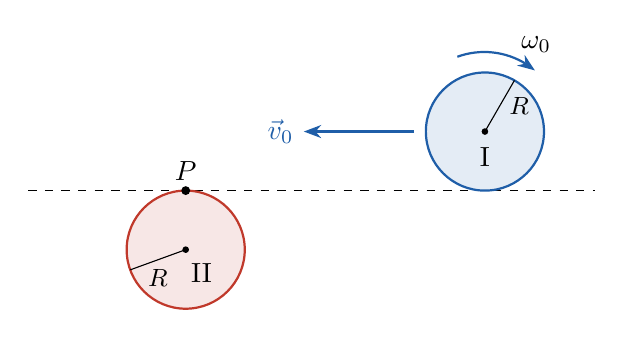
\begin{tikzpicture}[scale=1.0]
  \draw[dashed] (-0.6,0) -- (6.6,0);
  \draw[thick, azul, fill=azul!12] (5.2,0.75) circle (0.75);
  \fill (5.2,0.75) circle (1.2pt);
  \draw (5.2,0.75) -- ++(60:0.75) node[midway, right, font=\small]{$R$};
  \node at (5.2,0.42) {I};
  \draw[->, thick, azul] (4.3,0.75) -- (2.9,0.75) node[left]{$\vec{v}_0$};
  \draw[->, thick, azul] (4.85,1.7) arc[start angle=110, end angle=50, radius=1.0];
  \node at (5.85,1.85) {$\omega_0$};
  \draw[thick, rojo, fill=rojo!12] (1.4,-0.75) circle (0.75);
  \fill (1.4,-0.75) circle (1.2pt);
  \draw (1.4,-0.75) -- ++(200:0.75) node[midway, below, font=\small]{$R$};
  \node at (1.6,-1.05) {II};
  \fill (1.4,0) circle (1.6pt) node[above]{$P$};
\end{tikzpicture}
\end{document}
